\chapter{Analyse und Auswertung}\label{analysis}


\section{Testsystem}

Die Performanztests wurden auf einem Vierkernprozessor Intel i5-4590 mit 8GB Arbeitsspeicher durchgeführt.


\section{Analyse mit Valgrind}

In diesem Abschnit wird auf die Analyse des Projektes mit Valgrind eingegangen. Zunächst werden Valgrind und die daraus benutzten Tools vorgestellt und dann werden einige Ergebnisse präsentiert.
\subsection{Valgrind}

Valgrind ist einerseits ein Framework zum Erzeugen von dynamsichen Analyse Werkzeugen und andereseits eine Sammlung ebensolcher Werkzeuge (siehe \cite{10.1145/1250734.1250746}). 
Valgrind ist offene Software und wird unter der GNU GPL-2 Lizenz veröffentlicht\footnote{\url{https://valgrind.org/}}.
Die Sammlung bietet acht Werkzeuge\footnote{vgl. \url{https://valgrind.org/info/tools.html}} an von denen eines noch den Status eines experimentellen Werkzeugs hat:
\begin{itemize}
  \item Memcheck, ein Werkzeug zum Analysieren von Speicherlecks.
  \item Cachegrind, ein Cache und Branch-prediction Profiler.
  \item Callgrind, ein Profiler der einen Aufrufgraphen erzeugt.
  \item Helgrind und DRD, Werkzeuge um Threading-Fehler zu erkennen.
  \item Massif und DHAT, Heapprofiler für Analysen hinsichtlich speichereffizienter Programme 
  \item BBV, ein Werkzeug Forschung im Bereich der Rechnerarchitektur
\end{itemize}

In dieser Arbeit wurden die Werkzeuge Memcheck, Cachegrind und Callgrind verwendet. Die Ergebnisse der Werkzeuge DRD und Helgrind waren unbrauchbar, da diese nicht mit oneTBB kompatibel waren.

\subsubsection{cachegrind und callgrind}

Cachegrind und Callgrind, entwickelt von \citeauthor{Weidendorfer2004ATS}, sind sogenannte Cacheprofiler. 
Diese Werkzeuge werden verwendet um die Programmstellen mit der größten Laufzeit festzustellen und verschiedene Umstellungen im Programmcode vergleichen zu können.

Cachegrind simuliert wie das zu testende Programm mit der Cache-Hierarchie und dem Branch-Predictor einer virtuellen Maschine interagiert. Die dabei simulierte Maschine ist orientiert and der Architektur moderner Maschinen.
Dabei werden verschiedene Caches simuliert und die Zugriffe darauf hinsichtlich von Misses ausgewertet. In Abbildung \ref{callgrind} ist ein Beispielaufruf zu sehen.
 

\begin{figure}
  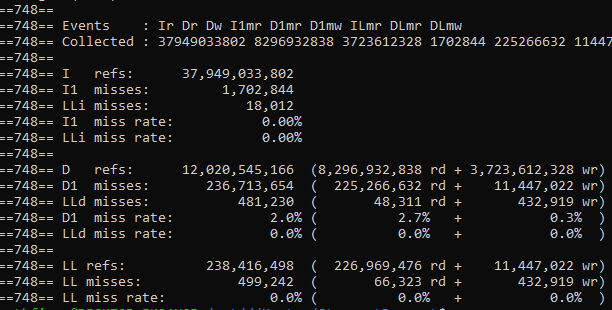
\includegraphics{images/callgrind.png}
  \caption{Beispielaufruf von Callgrind}\label{callgrind}
\end{figure}
%\subsubsection{Memcheck}

%Gehört eigentlihc nciht wirklcih hier her
%Screenshot plus was macht das Tool. Wir haben das genutzt um sicherzustellen, dass es keine Memoryleaks gibt.

\subsubsection{Auswerten von callgrind-Ergebnissen}


Mithilfe der Anwendung QCachegrind können die Ergebnisse von Valgrinds cachegrind/callgrind grafisch ausgewertet werden. QCachegrind ist ein Windowsbuild der Opensource Anwendung KCacheGrind.
KCachegrind ist Teil der Werkzeuge aus der Arbeit \cite{Weidendorfer2004ATS}.

\begin{figure}
  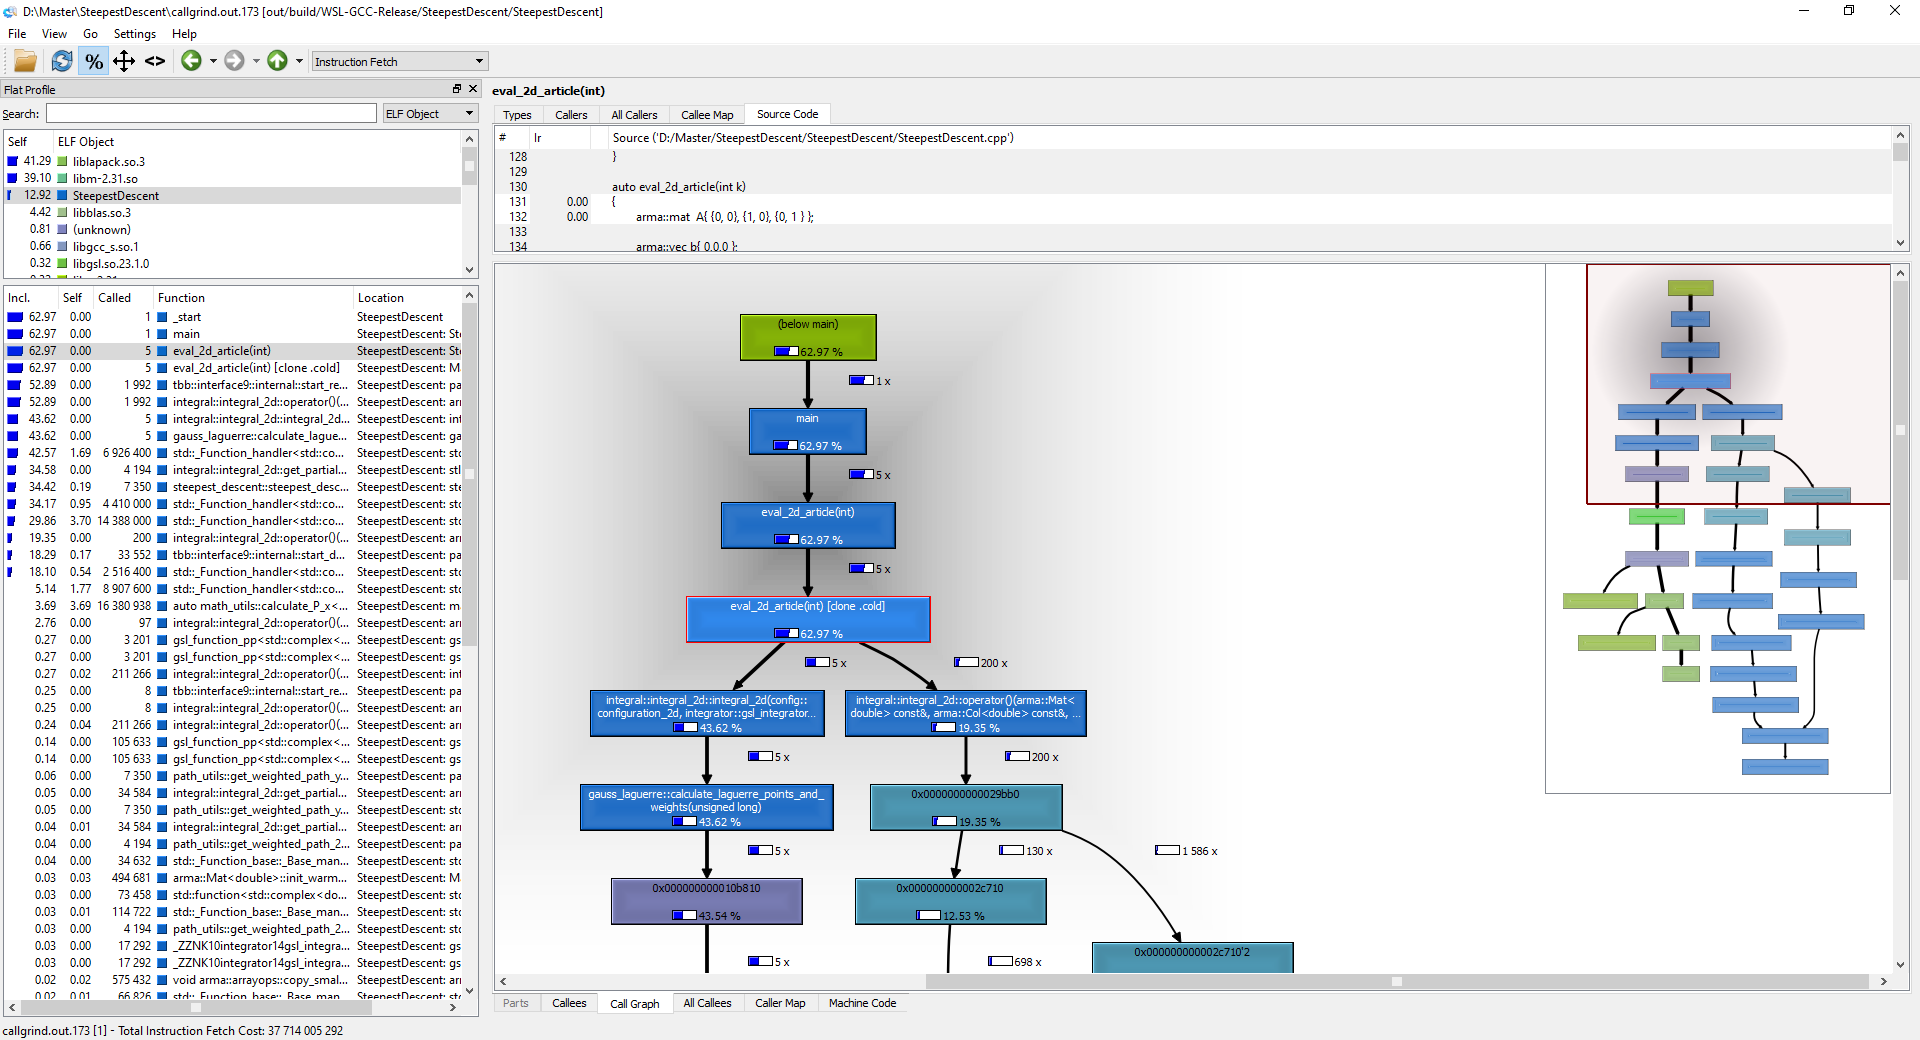
\includegraphics[width=\textwidth]{images/qcachegrind.png}
  \caption{Übersicht von QCachegrind}\label{qcachegrind}
\end{figure}

In Abbildung \ref{qcachegrind} ist eine Übersicht einer Auswertung mit QCachegrind zu sehen. In diesem Beispiel wurde mithilfe des Werkzeugs \texttt{callgrind} eine Aufzeichnung des zweidimensionalen Falls 
mit verschiedenen Wellenzahlen und jeweils 40 Stichproben von Beobachtungspunkt und Richtungsektoren für ein festes Dreieck berechnet.
Abbildung \ref{qcachegrind_result} zeigt einen Ausschnitt des Aufrufgraphen vergrößert dar. In diesem lassen sich an Pfeilen ablesen wie oft welcher Programmteil aufgerufen wird und mithilfe einer prozentualen Angabe einsehen wie viel der Laufzeit in diesem Teil verbraucht wird.

\begin{figure}
  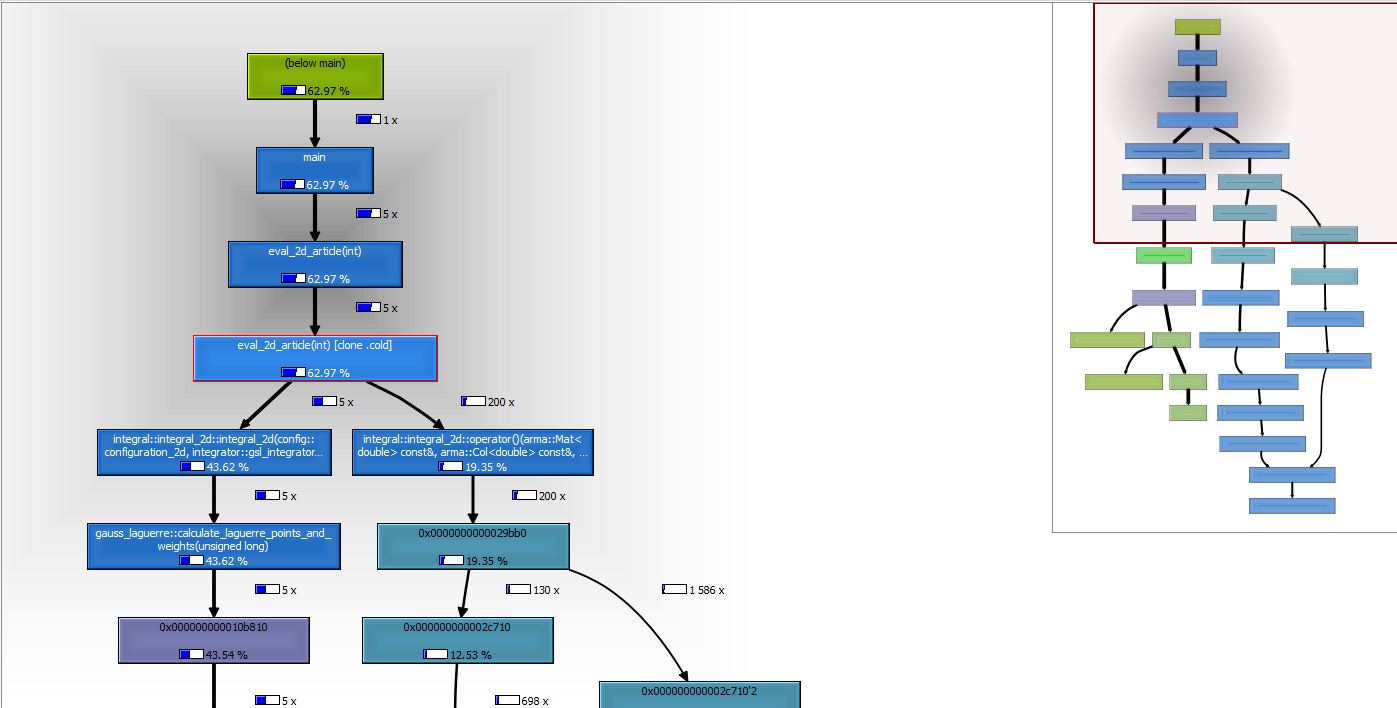
\includegraphics[width=\textwidth]{images/qcachegrind_callgraph.png}
  \caption{Aufrufgraph aus QCachegrind}\label{qcachegrind_result}
\end{figure}

Aus diesen und weiteren Auswertungen werden die meistaufgerufene Funktion und der Hotpath ersichtlich.

\section{Ergebnisse der Optimierungsmaßnahmen}

In diesem Abschnitt wird auf einige Ergebnisse der manuellen Performance-Messungen eingegangen.

\subsection{Hotpath}

Der häufigste Fall der Anwendung ist das Berechnen des Integrals in Situationen in denen keine Singularität auftritt. 
Dementsprechend werden diese in den implementierten Funktionen als der regelfall betrachtet.
Durch das vorziehen der Codestellen die diese Szenarien abhandeln werden beispielsweise die benötigten Sprunganweisungen geringer gehalten.



\subsection{Meistaufgerufene Funktion}

Die Funktion mit der größten Laufzeit ist das \textit{Steepest-descent}-Verfahren.
Diese Funktion ist über mehrere Iterationen optimiert worden, bis sie die im Kapitel \ref{Implementierung} dargestellte Form erreichte.
In früheren Versionen war dieses Verfahren in einer eigenen C++-Klasse implementiert, allerdings haben die Auswertungen gezeigt, dass ein
direkterer Aufruf der Gauss-Laguerre-Quadratur einen Laufzeitgewinn von fast 50 Prozent erzielen lies.

\subsection{Vermeiden von Funktionsaufrufen}

Bei der Implementierung des zweidimensionalen Falls \ref{2dint} hat sich gezeigt, dass das Nutzen der eindimenisionalen Implementierung zu erhöhten Laufzeiten geführt hat.

In diesem Test wird die Laufzeit hinsichtlich veränderter Auflösung $res \in \{ 0.1, 0.01, 0.001, 0.0001 \}$ gemessen.
Für jedes $k$ werden 50 zufällige Richtungsvektoren $r$ berechnet mit 600 Gauss-Laguerre-Knoten berechnet.

\begin{equation}
  A = \begin{pmatrix}
      0 & 0 \\
      1 & 0 \\
      0 & 1 \\
  \end{pmatrix}, b = \begin{pmatrix}
      0 \\ 0\\ 0
  \end{pmatrix},
\end{equation}

Veränderung: läuft über resoltuion nicht K!s

Diese Messungen werden in der Abbildung \ref{abb_perf_indirect} dargestellt.

\begin{center}
  
\end{center}

Grafik folgt noch

\section{Auswertung der Laufzeitmessugen}

Die folgenen Laufzeitvergleiche wurden aus einer Matlab Umgebung heraus ausgeführt, d.h. es werden die ursprüngliche Implementierung sowie das Matlab-Modul der C++ Implementierung verglichen.


\subsection{Iteration über Wellenzahl}


In diesem Test wird die Laufzeit hinsichtlich veränderter Wellenzahl $k \in \{ 100, 500, 1000, 3000, 5000 \}$ gemessen.
Für jedes $k$ werden 50 zufällige Richtungsvektoren $r$ berechnet mit 600 Gauss-Laguerre-Knoten berechnet.

\begin{equation}
  A = \begin{pmatrix}
      0 & 0 \\
      1 & 0 \\
      0 & 1 \\
  \end{pmatrix}, b = \begin{pmatrix}
      0 \\ 0\\ 0
  \end{pmatrix},
\end{equation}

\begin{center}
    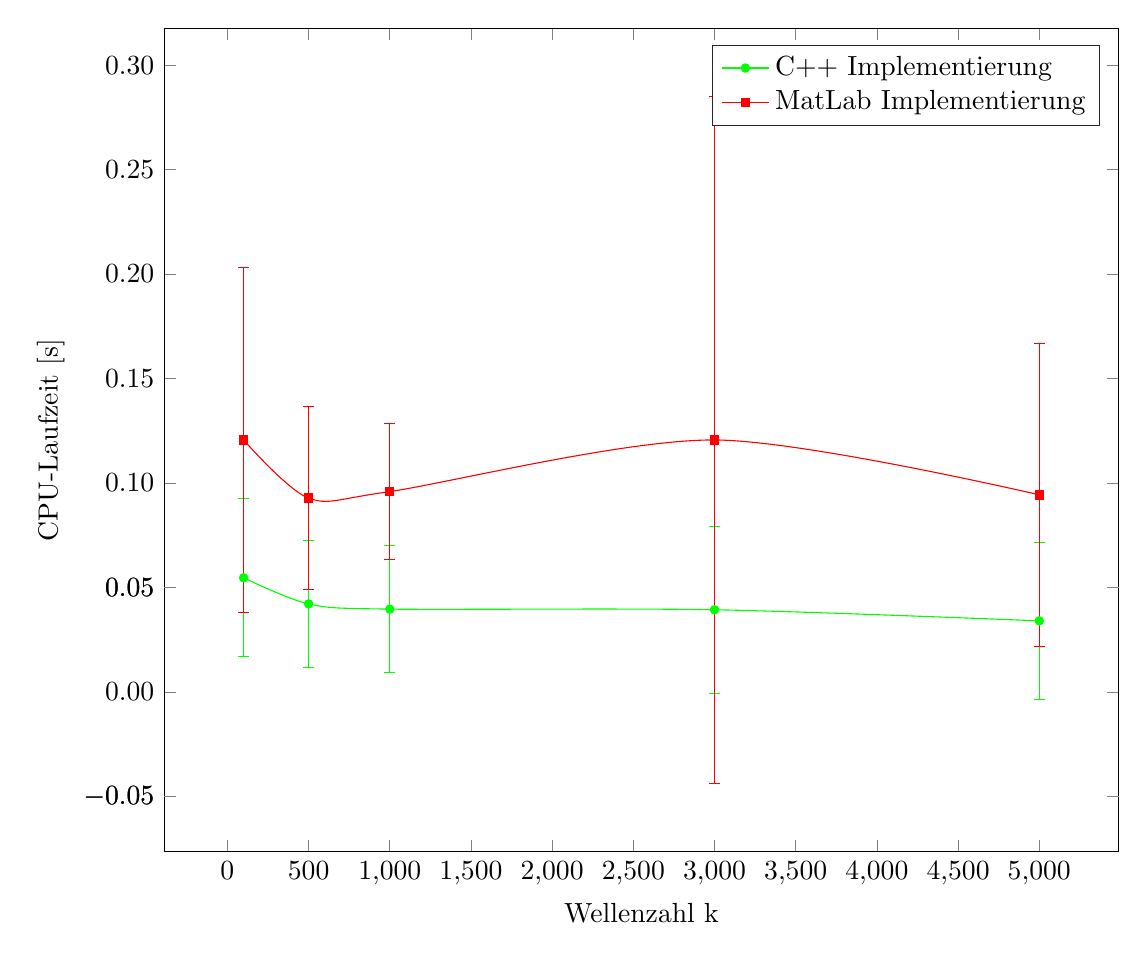
\begin{tikzpicture}
        \begin{axis}[
          width=\textwidth,
                  %width=3.358in,
        %height=2.309in,
        %at={(0.563in,0.312in)},
        scale only axis,
        yticklabel style={
          /pgf/number format/fixed,
          /pgf/number format/precision=2,
          /pgf/number format/fixed zerofill
        },
        extra y ticks={-0.05, 0.05},
        scaled y ticks=false,
        xlabel=Wellenzahl k,
        ylabel=\text{CPU-Laufzeit [s]},
        %xmin=0,
       % xmax=6000,
        %ymin=0,
        %ymax=0.5,
        axis background/.style={fill=white},
        legend style={legend cell align=left, align=left, draw=white!15!black}
        ]
        \addplot+[
      green, mark options={green, scale=0.75},
      smooth, 
      error bars/.cd, 
        y fixed,
        y dir=both, 
        y explicit ] table [color=green, mark=o, mark options={solid, green} x=k, y=t,y error=std, col sep=comma] { 
            k, t, std 
            100, 0.0546875000000000, 0.0377819439281490
            500, 0.0421875000000000, 0.0304832595619367
            1000, 0.0396875000000000, 0.0304767208961468
            3000, 0.0393750000000000, 0.0399597214296433
            5000, 0.0340625000000000, 0.0374428241844571         
          };
          \addplot+[
            red, mark options={red, scale=0.75},
            smooth, 
            error bars/.cd, 
              y fixed,
              y dir=both, 
              y explicit ] table [color=red, mark=o, mark options={solid, red} x=k, y=t,y error=std, col sep=comma] { 
                  k, t, std 
                  100, 0.120625000000000, 0.0825011595465820
                  500, 0.0928125000000000, 0.0439012055439740
                  1000, 0.0959375000000000, 0.0326549607327770
                  3000, 0.120625000000000, 0.164181352722021
                  5000, 0.0943750000000000, 0.0724645849462240          
                };
        %\addplot [color=red, draw=none, mark=o, mark options={solid, mycolor1}]
        %  table[row sep=crcr] file {..\data\performance_matlab.csv};
        \addlegendentry{C++ Implementierung}
        \addlegendentry{MatLab Implementierung}

        \end{axis}
    \end{tikzpicture}%
    \captionof{figure}{Laufzeitvergleich über verschiedene Wellenzahlen $k$}
\end{center}


\subsection{Laufzeitvergleich bei steigender Auflösung}


In diesem Test wird die Laufzeit hinsichtlich veränderter Auflösung $res \in \{ 0.1, 0.01, 0.001, 0.0001 \}$ gemessen.
Für jedes $k$ werden 50 zufällige Richtungsvektoren $r$ berechnet mit 600 Gauss-Laguerre-Knoten berechnet.

\begin{equation}
  A = \begin{pmatrix}
      0 & 0 \\
      1 & 0 \\
      0 & 1 \\
  \end{pmatrix}, b = \begin{pmatrix}
      0 \\ 0\\ 0
  \end{pmatrix},
\end{equation}
    
\begin{center}
    \begin{tikzpicture}
        \begin{axis}[
        %width=3.358in,
        %height=2.309in,
        %at={(0.563in,0.312in)},
        scale only axis,
        xmode=log,
        ymode=log,
        ymax=1000,
        width=\textwidth,
        %log ticks with fixed point,
        x dir=reverse,
        ylabel=\text{CPU-Laufzeit [s] (log)},
        xlabel=Layer-Auflösung (log),
        % for log axes, x filter operates on LOGS.
        % and log(x * 1000) = log(x) + log(1000):
        %x filter/.code=\pgfmathparse{#1 + 6.90775527898214},
        axis background/.style={fill=white},
        legend style={legend cell align=left, align=left, draw=white!15!black}
        ]
        \addplot+[
      green, mark options={green, scale=0.75},
      smooth, 
      error bars/.cd, 
        y fixed,
        y dir=both, 
        y explicit ] table [color=green, mark=o, mark options={solid, green} x=res, y=t,y error=std, col sep=comma] { 
            res, t, std
            0.1000,    0.0563,    0.0461
            0.0100,    0.3469,    0.0645
            0.0010,   3.8547,    1.6996
            0.0001,  38.9781,   15.6876
          };
          \addplot+[
            red, mark options={red, scale=0.75},
            smooth, 
            error bars/.cd, 
              y fixed,
              y dir=both, 
              y explicit ] table [color=red, mark=o, mark options={solid, red} x=res, y=t,y error=std, col sep=comma] { 
                  res, t, std
                  0.1000,    0.1375,    0.0799
                  0.0100,    0.8688,    0.0834
                  0.0010,    9.5406,    4.2787
                  0.0001,   86.2375,   27.7633
                };
        %\addplot [color=red, draw=none, mark=o, mark options={solid, mycolor1}]
        %  table[row sep=crcr] file {..\data\performance_matlab.csv};
        \addlegendentry{C++ Implementierung}
        \addlegendentry{MatLab Implementierung}
        \end{axis}
    \end{tikzpicture}%
    \captionof{figure}{Laufzeitvergleich über verschiedene Auflösungen, logarithmische Skalen}
\end{center}


\section{Vergleiche der Genauigkeit}

Auf das Fehlerszenarion eingehen.
Graph mit dem Fehlervergleich

Daten des relativen Fehlers messen 
=> matlab um die 7-e18 
=> gsl um die 1-e18

Das einfach mal auf einem Lauf rennen lassen

